\begin{columns}[totalwidth=.85\linewidth]
    \column{\textwidth}
    \vspace{-10mm}
        \begin{itembox}[l]{初期構造の作成\cite{sasaki}}
            \begin{enumerate}
                \item \alert{実空間}で8-Chain Model から初期構造を作成。
                    \begin{itemize}
                        \normalsize
                        \item 所望の分岐数に\alert{ランダム}に選択した\alert{結合を除去}
                        \item 除去したジオメトリーに対応した\alert{トポロジーモデル}
                    \end{itemize}
                \item トポロジー空間でランダム性の導入
                    \begin{itemize}
                        \normalsize
                        \item \alert{エッジ交換}して、ノードごとにランダムな接続性を導入
                    \end{itemize}	
                \item 対応する\alert{実空間でのネットワーク初期構造}を作成
                \item \alert{ストランド長がホモポリマーに対応}するように多重度設定
                \item \alert{Slow Push Off\cite{auhl} により初期構造を緩和}
            \end{enumerate}

            \vspace{-1mm}
            \begin{columns}[T, onlytextwidth]
                \column{.33\linewidth}
                    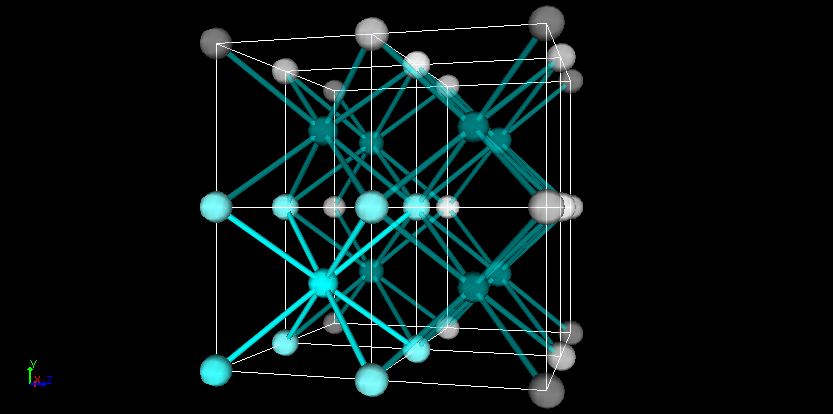
\includegraphics[width=\textwidth]{8_per.png}
                \column{.33\linewidth}
                    \vspace{-5mm}
                    \begin{center}
                        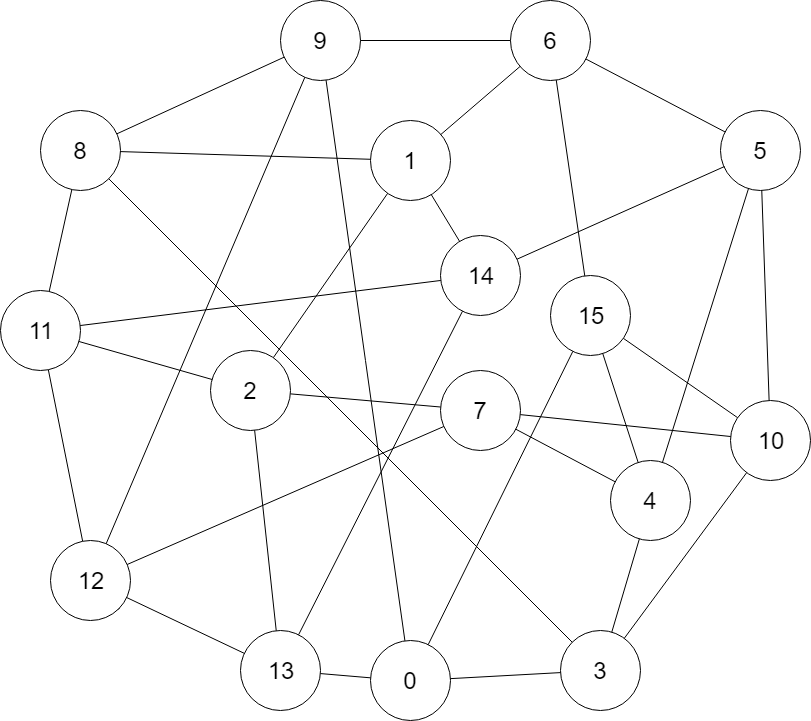
\includegraphics[width=.6\textwidth]{Network.png}
                    \end{center}
                \column{.33\linewidth}
                    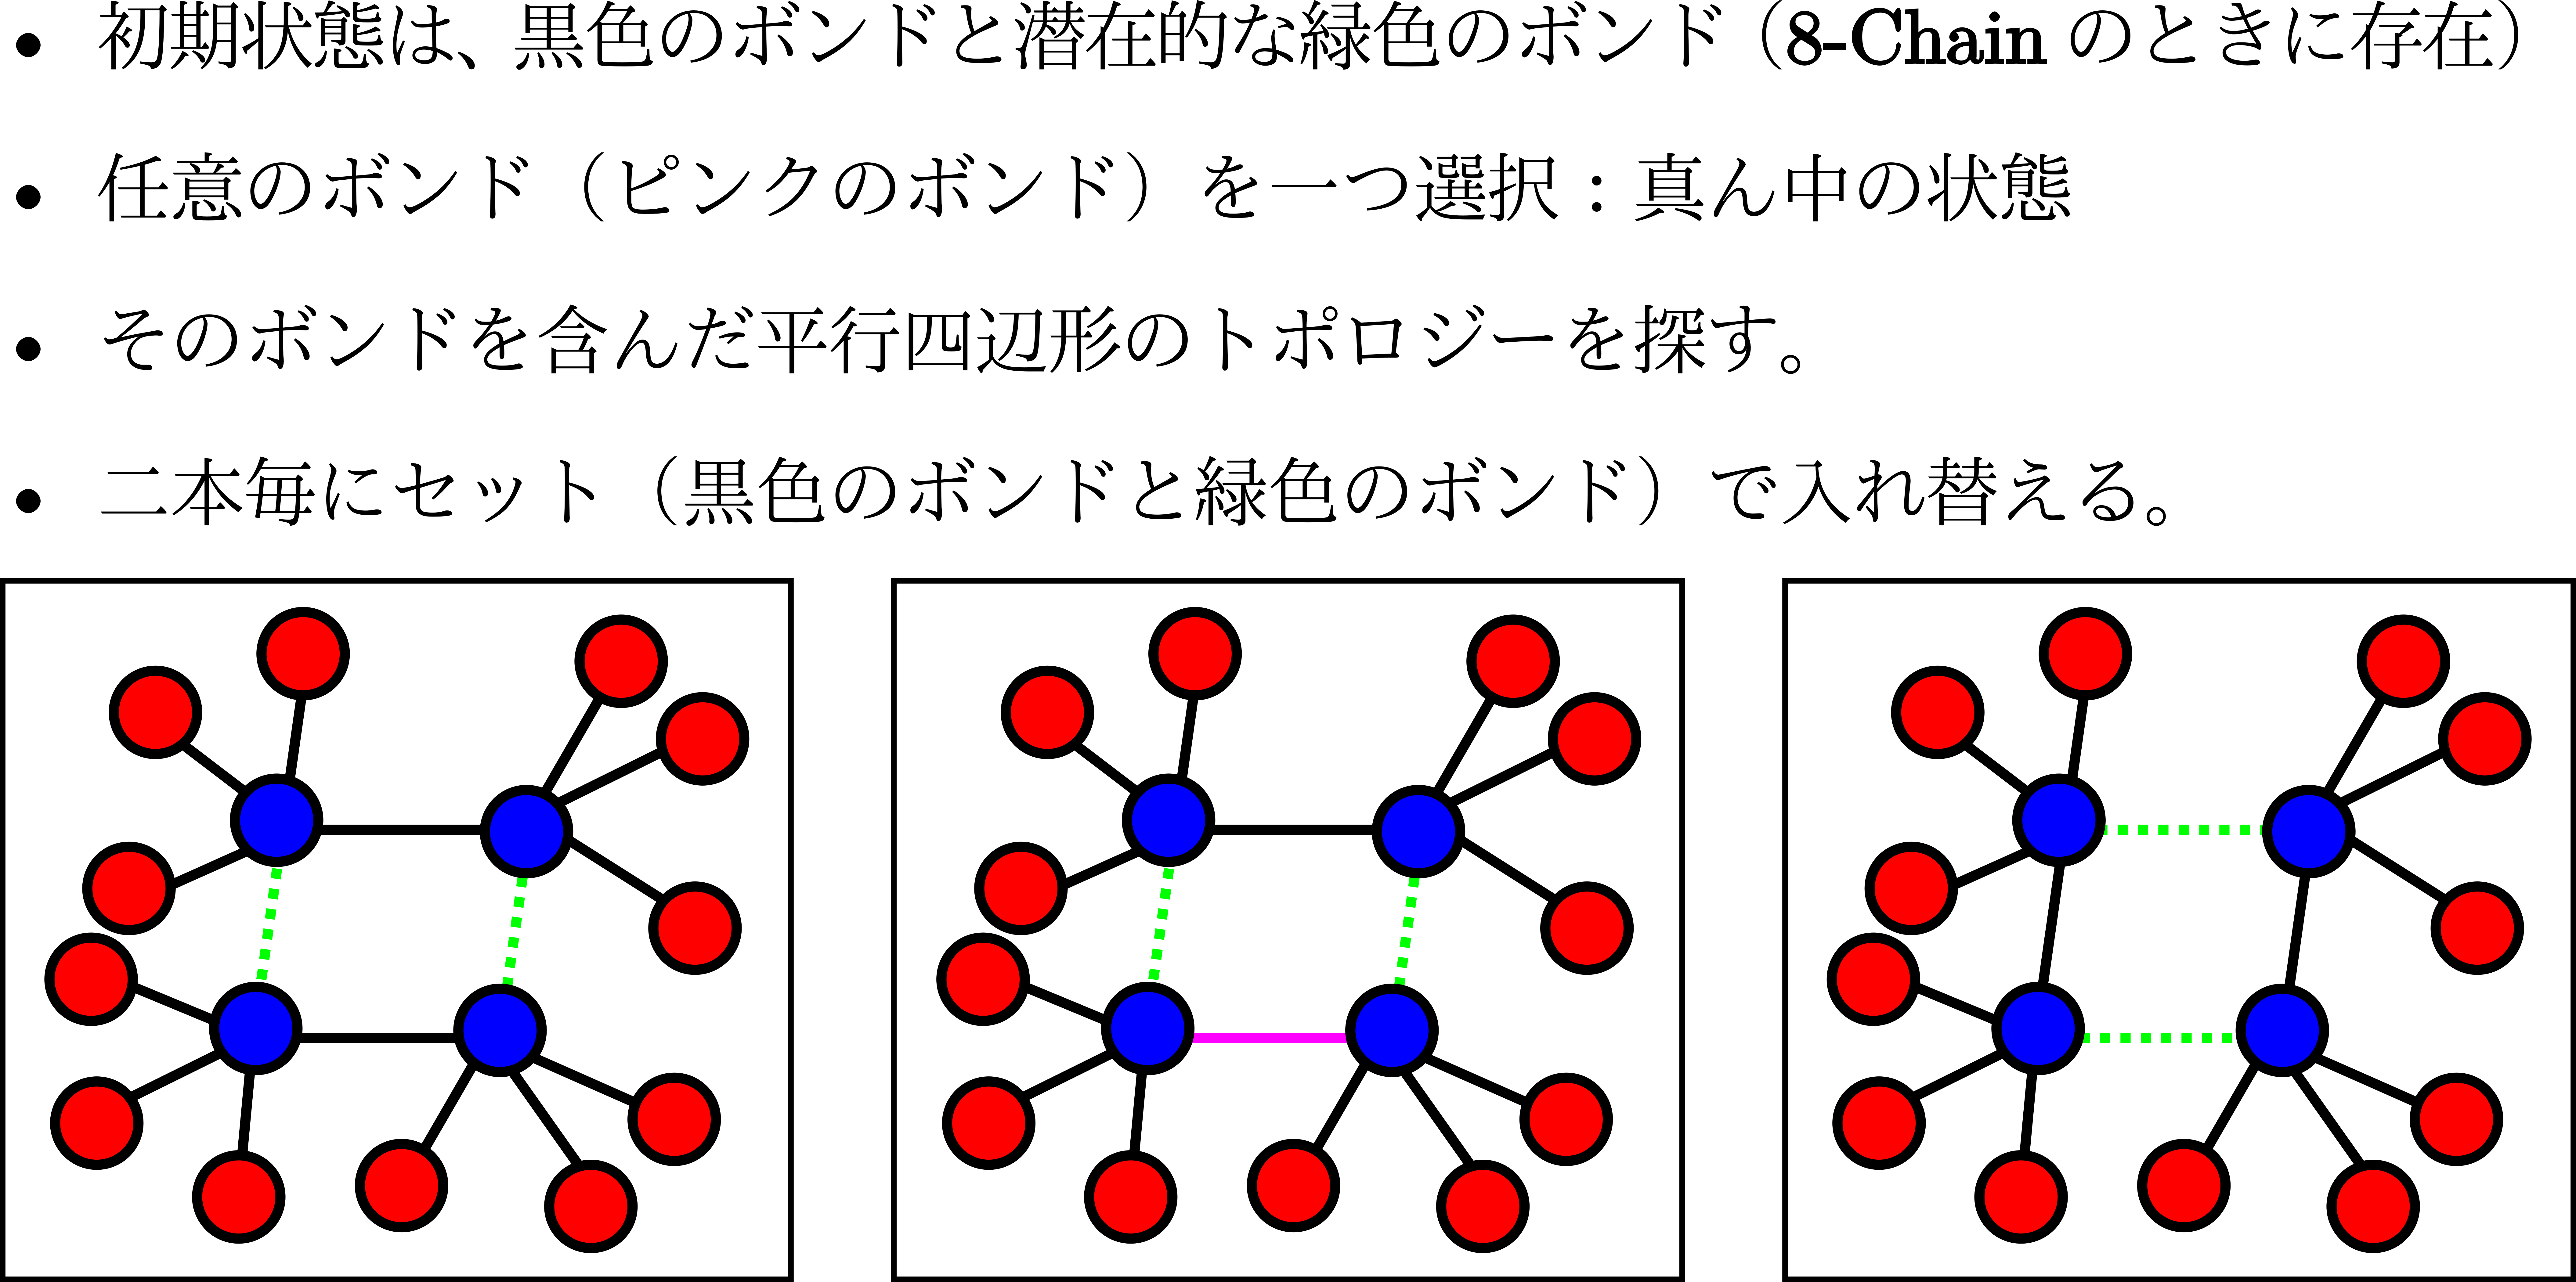
\includegraphics[width=\textwidth]{bond_exchg.png}
            \end{columns}
        \end{itembox}

        \begin{itembox}[l]{各種特性の評価}
            \begin{enumerate}
                \item 初期構造の確認
                    \begin{itemize}
                        \normalsize
                        \item Kr\"{o}ger らの方法~\cite{kroger} により Z\_1 Code で絡み合いを評価
                        \item 対応するホモポリマーメルトと同程度であることを確認
                    \end{itemize}
                \item 力学特性の評価
                    \begin{itemize}
                        \normalsize
                        \item Lees-Edwards 条件によりずりせん断を付与し、生じる応力を評価
                        \item 連続した変形を付与して、ヒステリシスを評価
                    \end{itemize}	
            \end{enumerate}
        \end{itembox}
\end{columns}